\subsection{Dispersion L\"uscher in 2 dimensions}

The discussion above is valid only in the continuum.
For a discretized lattice, an additional length scale is introduced that must be accounted for.
As is the case in both 3-D and 1-D, there exists a dispersion L\"uscher equation that is valid for the contact interaction and accounts for the discretization.
In \Appref{counterterm/dispersion} we derive this dispersion L\"uscher formula for 2D and only state the result here.

Identifying the lattice spacing $\epsilon=N/L$, we have
\begin{align}
    \frac{2}{\pi} \log \left(\frac{2\pi \tilde a_{20}}{L}\right)
    &=
    \frac{1}{\pi^2}
    \left(
        \sum_{n_x,n_y=-\frac{N}{2}}^{\frac{N}{2}-1}\frac{1}{\frac{L^2}{4\pi}K_{nn}-x}
        -2\pi \log \left(\mathcal{L}_\square\frac{N}{2}\right)
    \right)
    \nonumber\\
    &\equiv\frac{1}{\pi^2}S^{\dispersion}_2\left(x\right)\ ,\label{eq:2d dispersion luscher}
\end{align}
where $x$ is defined as usual,
\begin{equation}
    \mathcal{L}_{\square}
    =
    \exp \left(\log (2)-G \frac{2}{\pi}\right)
    =
    1.116306393581637659468497 \ldots
\end{equation}
and $G$ is Catalan's constant.

Given a contact interaction with coefficient appropriately tuned to the continuum scattering length $\tilde a_{20}$ and accounts for the discretization $\epsilon=N/L$ (see \Appref{counterterm/dispersion}),
\begin{equation}
C(N/L)=-\frac{2 \pi}{m \log \left(\tilde a_{20} \mathcal{L}_\square \frac{N}{L}\pi\right)}\ ,
\end{equation}
the finite-spacing finite-volume energy eigenvalues of Schr\"odinger's equation on a square lattice will exactly satisfy the quantization condition \eqref{2d dispersion luscher}.

\todo{\@TOM: was this tuned using $S^{\spherical}$ or $S^{\dispersion}$? Am I getting your procedure right?}
To demonstrate the success of this formula we tuned lattices with $N=10$, 20, and 40 to $\tilde a_{20}/L = .1$, which allows for a bound state, using $S^{\dispersion}$.
In \Figref{luescher2d} the black points were analyzed through $S^\dispersion_2$, and lie on a flat line, indicating that our dispersion \Luscher formula has correctly accounted for discretization effects.
On the other hand, if we use the same energies but analyze them with the usual continuum \Luscher function $S^{\spherical}_2$, shown as colored points, we see induced momentum-dependence and the flat line behavior is lost.

\begin{figure}
    \center
    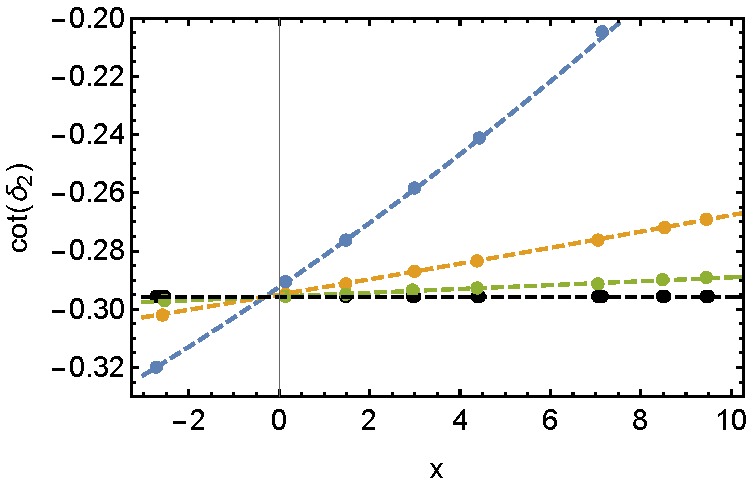
\includegraphics[width=.65\textwidth]{figure/luescher2d.pdf}
    \caption{
        Results in 2-D using non-continuum eigenvalues $x=p^2L^2/4\pi^2$ of the Schr\"odinger equation with $N=10$, 20, and 40.
        The interaction was tuned such that $\tilde a_{20}/L=.1$.
        The colored points are obtained using $S^\spherical_2(x)$ with $N=10$ being furthest from a flat line and $N=40$ being closest.
        The black points are obtained using $S^{\dispersion}_2(x)$ and exhibit the correct flat-line behavior.
        The colored dashed lines are the derived induced momentum-dependent terms (see text) \todo{Need better figure. -T.L.}}
    \label{fig:luescher2d}
\end{figure}

As was done in the 3-D\todo{still needs to be done.-T.L.} and 1-D cases, we can derive the functional form of the induced momentum-dependent terms.  The steps are identical to those done in the 3-D and 1-D cases, and so for conciseness we show only the end result.  Assuming an $x=\left(\frac{pL}{2\pi}\right)^2$ calculated on a \emph{discretized} lattice with lattice spacing $\epsilon=N/L$, we have
\begin{align*}
 \frac{1}{ \pi^{2}} S^\bigcirc_{2}\left(x\right)&=\frac{2}{\pi}\log\left(2\pi \frac{\tilde a_{20}}{L}\right)+ \frac{1}{ \pi^{2}} S^\bigcirc_{2}\left(x\right)- \frac{1}{ \pi^{2}} S^{\dispersion}_{2}\left(x\right)\\
 &=\frac{2}{\pi}\log\left(2\pi \frac{\tilde a_{20}}{L}\right)+\frac{1}{\pi^{2}} \left(\lim_{\eta\to\infty}\sum_{n\notin \operatorname{B.Z.}}^{|n|\le\frac{\eta}{2}} \frac{1}{n^{2}-x} -2\pi\log\left(\frac{\eta}{\mathcal{L}_\square N}\right)\right)\\
&=\frac{2}{\pi}\log\left(2\pi \frac{\tilde a_{20}}{L}\right)+\frac{1}{\pi^{2}} \left(\lim_{\eta\to\infty}\sum_{n\notin \operatorname{B.Z.}}^{|n|\le\frac{\eta}{2}}  \frac{1}{n^{2}} -2\pi\log\left(\frac{\eta}{\mathcal{L}_\square N}\right)\right)
+\frac{1}{\pi^{2}}\sum_{n\notin \operatorname{B.Z.}} \frac{x}{n^{4}} +\frac{1}{\pi^{2}}\sum_{n\notin \operatorname{B.Z.}} \frac{x^2}{n^{6}}+\mathcal{O}(x^3)\\
&\equiv\frac{2}{\pi}\log\left(2\pi \frac{\tilde a_{20}}{L}\right)+\alpha_0(N)+\alpha_1(N) x+\alpha_2(N) x^2 +\mathcal{O}(x^3) \ .
\end{align*}
The coefficients $\alpha_i(N)$ have an implicit dependence on $N$ since the sums are restricted outside of the Brillouin zone.  Further, in 2-D the sums involved in $\alpha_i$ converge sufficiently fast and thus require no acceleration techniques.  We provide
\begin{table}
\caption{The induced momentum-dependent terms to order $x^2$ due to a contact interaction using $S^\bigcirc_2(x)$ as a function of discretization $N$.  Here $x=\left(\frac{pL}{2\pi}\right)^2$ is a non-continuum eigenenergy.  \label{tab:induced terms in 2 d}}
\begin{tabular}{c|c}
$N$ & $\alpha_0(N)+\alpha_1(N) x+\alpha_2(N) x^2$\\
\hline
10 &$0.003446926 + 0.01065059589 x + 0.00018852319 x^2$\\
20 &$0.000862459 + 0.00261909878 x + 0.00001122531 x^2$ \\
40 &$0.000212552 + 0.00065179064 x + 6.92648\times10^{-7} x^2$ \\
\hline
\end{tabular}
\end{table}
the numerical values of $\alpha_i(N)$ in \autoref{tab:induced terms in 2 d} for the discretizations shown in \autoref{fig:luescher2d}.  They were also used to calculate the dashed colored lines in \autoref{fig:luescher2d}.
